\documentclass{article}
\usepackage[utf8]{inputenc}
\usepackage{subfig}

%References
\usepackage{natbib}
%IMPORTANT use https://www.citationmachine.net/ if you need to generate references!
% \citep{reference} creates Harvard Style references throughout

%Colors
\usepackage{xcolor}

\usepackage[protrusion=true,expansion]{microtype}

%Code Markup
\usepackage[outputdir=cache]{minted}
%Syntax Highlighting Style
\definecolor{bggray}{RGB}{40,40,40}
\newmintedfile[javacode]{java}{
	style=fruity,
	bgcolor=bggray,
	linenos,
	breaklines,
	tabsize=2,
	obeytabs
}

\newmintedfile[bashoutput]{text} {
	style=fruity,
	bgcolor=bggray,
	breaklines,
	tabsize =2,
	obeytabs
}

\newmintedfile[armfile]{ARM} {
	style=fruity,
	bgcolor=bggray,
	breaklines,
	tabsize =2,
	obeytabs
}

%Page Margins and stuff
\usepackage{geometry}
 \geometry{
 a4paper,
 total={170mm,257mm},
 left=20mm,
 }

%Pictures
\usepackage{graphicx}
\graphicspath{ {./images/} }

%Move the title position
\usepackage{titling}

\setlength{\droptitle}{-8.5em} %Up, near the top but not too high

\title{Assignment 1 - CT2109 Object Oriented Programming: Data Structures and Algorithms}
\author{Daniel Hannon (19484286)}
\date{Feburary 2021}

\begin{document}
	\maketitle
	%Sets to Harvard Style and links the references file
	\section{Problem Analysis}
	\textit{Abstract: In this assignment, you will write a program for reading in the letters of the alphabet, one at a time, in order from the console. The user should press enter between each letter and incorrect letters in the sequence should be ignored. Once the user has typed the letters in the correct sequence, the program should tell them how long it took to complete. The user can also decide if they would like to type the letters forwards or backwards.} \\

	In order to achieve this I must come to grips with the \textbf{Scanner} Class.\\
	I must be able to also be able to use the \textbf{Date} Class.\\
	As this reads one letter at a time, I want to make sure that words starting with the expected letter do not qualify as valid input, This can easily be achieved by:
	\begin{itemize}
		\item Using \textbf{String.stringify(}\textit{startIndex,endIndex}\textbf{)}
		\item Using \textbf{String.equals(}\textit{anotherString}\textbf{)} in conjunction with the afforementioned method
	\end{itemize}
	I felt that there was no need for it to be case sensitive so I utilized \textbf{Scanner.nextLine().toLowerCase()} to guarantee it was always lowercase.
	\\ I stored the alphabet as a string either forwards or backwards depending on the initial input. I then invoke \textbf{String.stringify(}\textit{position,(position + 1)}\textbf{)} to get the current letter if \textbf{String.equals(}\textit{otherString}\textbf{)} evaluates to true, then \textit{position} is incremented.\\
	Once \textit{position} is equal to the length of the Alphabet string, it breaks.
	\\Time keeping is done as follows
	\begin{itemize}
		\item Initialize \textit{date} to value \textbf{new Date()}
		\item Create a long called \textit{totalTime}
		\item Set it's value to the value \textbf{date.getTime()}
		\item Once the input is complete reinitialize date to \textbf{new Date()}
		\item Perform the operation \textit{totalTime = \textbf{date.getTime()} - totalTime}
		\item Display the result.
	\end{itemize}
	By using \textbf{String.equals()} I am ultimately eliminating the need for \textbf{String.length()} as it will always be compared to a string of length 1
	\newpage
	\section{Code}
	\javacode{Main.java}
	\newpage
	\section{Testing}
	\subsection{Testing inital input}
	\begin{figure}[!h]
		\centering
		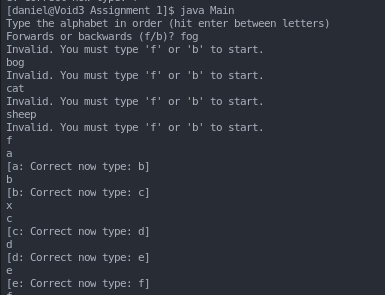
\includegraphics[width=\textwidth]{1.png}
	\end{figure}
	\newpage
	\subsection{Testing reverse and Caps}
		\begin{figure}[!h]
			\centering
			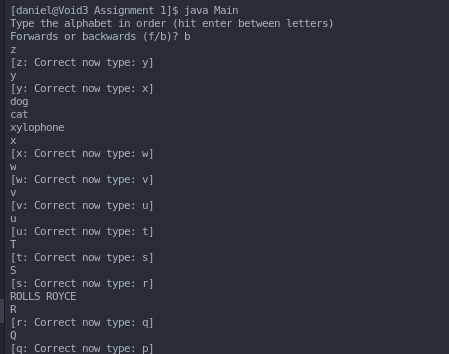
\includegraphics[width=\textwidth]{2.png}
		\end{figure}
		\newpage
	\subsection{Demonstration of Time}
		\begin{figure}[!h]
			\centering
			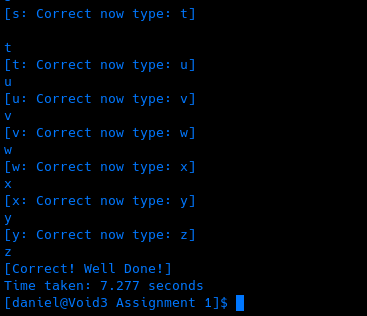
\includegraphics[width=\textwidth]{3.png}
		\end{figure}
	\bibliographystyle{agsm}
	\bibliography{references}
\end{document}
